\chapter{Διαχείριση Εργασιών}
    Καταρχάς είναι σημαντικό να αποσαφηνίσουμε την έννοια του προγραμματισμού και της παρακολούθησης εργασιών, μια διαδικασία που μπορούμε να ονομάσουμε ως διαχείριση εργασιών. Στο κεφάλαιο αυτό θα αναφερθούμε αναλυτικά στη διαδικασία αυτή, θα...
    
    \section{Το πρόβλημα της διαχείρισης εργασιών}

        \subsection{Εργασία}
    
        \subsection{Ορισμός της διαχείρισης εργασιών}
            Ως \textbf{διαχείριση εργασιών} (task management) θα χαρακτηρίζαμε την διαδικασία οργάνωσης, ιεράρχησης και παρακολούθησης των εργασιών (tasks) καθ' όλη τη διάρκεια μέχρι να πραγματοποιηθούν, με σκοπό την διασφάλιση της αποδοτικής και αποτελεσματικής εκτέλεσής τους.
            
            Πρόκειται για μια διαδικασία που είναι καθοριστικής σημασίας για τη βελτίωση της παραγωγικότητας, είτε σε ατομικό είτε σε συλλογικό επίπεδο. Μπορεί να γίνει χειροκίνητα, αλλά πλέον συχνά χρησιμοποιούνται ψηφιακά εργαλεία τα οποία αυτοματοποιούν διάφορες πτυχές της.
        
        \subsection{Πεδίο εφαρμογής διαχείρισης εργασιών}
            Η διαδικασία της διαχείρισης εργασιών έχει ένα ευρύ πεδίο εφαρμογής, καθώς εκτίνεται από απλές καθημερινές δραστηριότητες ως το χειρισμό πολύπλοκων χρονοβόρων εργασιών.        

            Η πιο εύληπτη εφαρμογή της αφορά τον καθημερινό προσωπικό προγραμματισμό των υποχρεώσεών μας. Αυτός περιλαμβάνει to-do λίστες, ημερολόγια ή απλές εφαρμογές (όπως Todoist, Notion ή το Google Keep) όπου οργανώνονται οι προσωπικές υποχρεώσεις, προγραμματίζονται ραντεβού ή δραστηριότητες αναψυχής, και εύκολα μπορούν να θέτονται βραχυπρόθεσμοι ή μακροπρόθεσμοι στόχοι και να παρακολουθείται η πρόοδός τους. \cite{Todoist} \cite{Notion}
            % TODO: Βελτιώνεται η ζωή των ατόμων καθώς πετυχαίνουν τις εργασίες τους και μειώνεται το άγχος τους

            Πέρα από το προσωπικό επίπεδο, μέθοδοι διαχείρισης έργων χρησιμοποιούνται ευρέως και σε επαγγελματικά περιβάλλοντα. Στόχος τους είναι η αποτελεσματική κατανομή του φόρτου εργασίας των εργαζομένων και η συντονισμένη συνεργασία τους. Μέσω της διαχείρισης έργων είναι ικανή η διευθέτηση παράλληλων εργασιών ταυτόχρονα, η ιεράρχησή τους σε επείγουσες και μη, η δίκαιη ανάθεση των εργασιών στους εργαζομένους κ.α. Ένα δημοφιλές εργαλείο που χρησιμοποιείται σε αυτά τα ομαδικά περιβάλλοντα είναι το Trello. \cite{Trello}

            Τέλος, με την πρόοδο της τεχνολογίας, έχουν δημιουργηθεί προηγμένες πλατφόρμες στις οποίες μπορεί να γίνει βελτιστοποίηση της ιεράρχησης εργασιών, χρησιμοποιώντας τεχνητή νοημοσύνη και ανάλυση δεδομένων. 

        \subsection{Διαφορά με διαχείριση έργου}
            Συχνά η έννοια της διαχείρισης εργασιών (task management) συγχέεται με αυτή της διαχείρισης έργου (project management). Η αλήθεια είναι πως πρόκειται για έννοιες που όντως συσχετίζονται αλλά στη πραγματικότητα η καθεμία εστιάζει σε διαφορετικά αντικείμενα.

            Η \textbf{διαχείριση εργασιών}, όπως έχει αναφέρθηκε, αφορά την παρακολούθηση διαφορετικών, μεμονομένων δραστηριοτήτων οι οποίες χρειάζεται να ολοκληρωθούν. Με άλλα λόγια εστιάζει περισσότερο στο \textit{μικροεπίπεδο}, στη διαχείριση καθημερινών υποχρεώσεων, στα διαφορετικά deadlines που μπορεί να υπάρχουν, την εξέλιξή τους ανά το χρόνο κ.α. Τα εργαλεία που αφορούν την διαχείριση εργασιών περιλαμβάνουν ημερολόγια, υπενθυμίσεις ή χρονοδιαγράμματα.

            Αντίθετα η \textbf{διαχείριση έργου} περιγράφει τον σχεδιασμό, την εκτέλεση και την ολοκλήρωση ενός ολόκληρου έργου. Ένα έργο αποτελείται και αυτό από διαφορετικές εργασίες, οι οποίες όμως είναι οργανωμένες προς έναν ευρύτερο στόχο. Επομένως η έννοια της διαχείρισης έργου \textit{συμπεριλαμβάνει} την διαχείριση εργασιών, αλλά επίσης προϋποθέτει επιπλέον απαιτήσεις όπως την σωστή κατανομή πόρων (resource allocation) ή την αξιολόγηση κινδύνου (risk assessment). Τα λογισμικά διαχείρισης έργου έχουν λειτουργικότητες όπως διαγράμματα Γκαντ, παρακολούθηση εξαρτήσεων κ.α.

            Στην παρούσα διπλωματική εργασία για λόγους πληρότητας θα αναλύσουμε κάποιες έννοιες που αφορούν και την διαχείριση έργου, έχοντας όμως υπόψην ότι η υλοποίηση αφορά την διαχείριση εργασιών.

    \section{Ιστορική αναδρομή}
        Είναι προφανές ότι η διαχείριση έργων δεν περιλάμβανε πάντα ψηφιακά εργαλεία και αυτοματισμούς. Πάντα όμως ήταν πρόδηλη σε όλα τα μεγάλα έργα της ιστορίας. Άλλωστε πώς αλλιώς θα μπορούσαν να ολοκληρωθούν τεράστια κατασκευάσματα όπως οι πυραμίδες της Αιγύπτου, το Στόουνχεντζ ή το Σινικό τείχος;
        
        Η έννοια της διαχείρισης έργων έδωσε την δυνατότητα στους ηγέτες να σχεδιάζουν τολμηρά και ογκώδη έργα και να κατανέμουν σωστά τα διαθέσιμα υλικά και ανθρώπους σε ένα καθορισμένο χρονικό διάστημα. 
        
        \subsection{Προφορικότητα και μνημονικές συσκευές}
            Στην αρχαιότητα η διαχείριση των εργασιών γινόταν προφορικά. Οι εργασίες αναθέτονταν και διαχειρίζονταν μέσω προφορικών οδηγιών, κάτι που σήμαινε πως μεγάλο ρόλο έπαιζε η ανθρώπινη μνήμη. \cite{Goody2013}

            Πολιτισμοί όπως οι Λούμπα του Κονγκό χρησιμοποιούσαν χειροκίνητες συσκευές όπως τη \textit{λουκάσα} (lukasa) που περιλάμβαναν πολύχρωμες χάντρες. Οι χάντρες ήταν τοποθετημένες σε συγκεκριμένες θέσεις, οι οποίες βοηθούσαν τη μνήμη την χειριστών ώστε να θυμηθούν την εκάστοτε πληροφορία και να οργανωθούν. \cite{Lukasa}

            \begin{figure}[H] \noindent \centering
                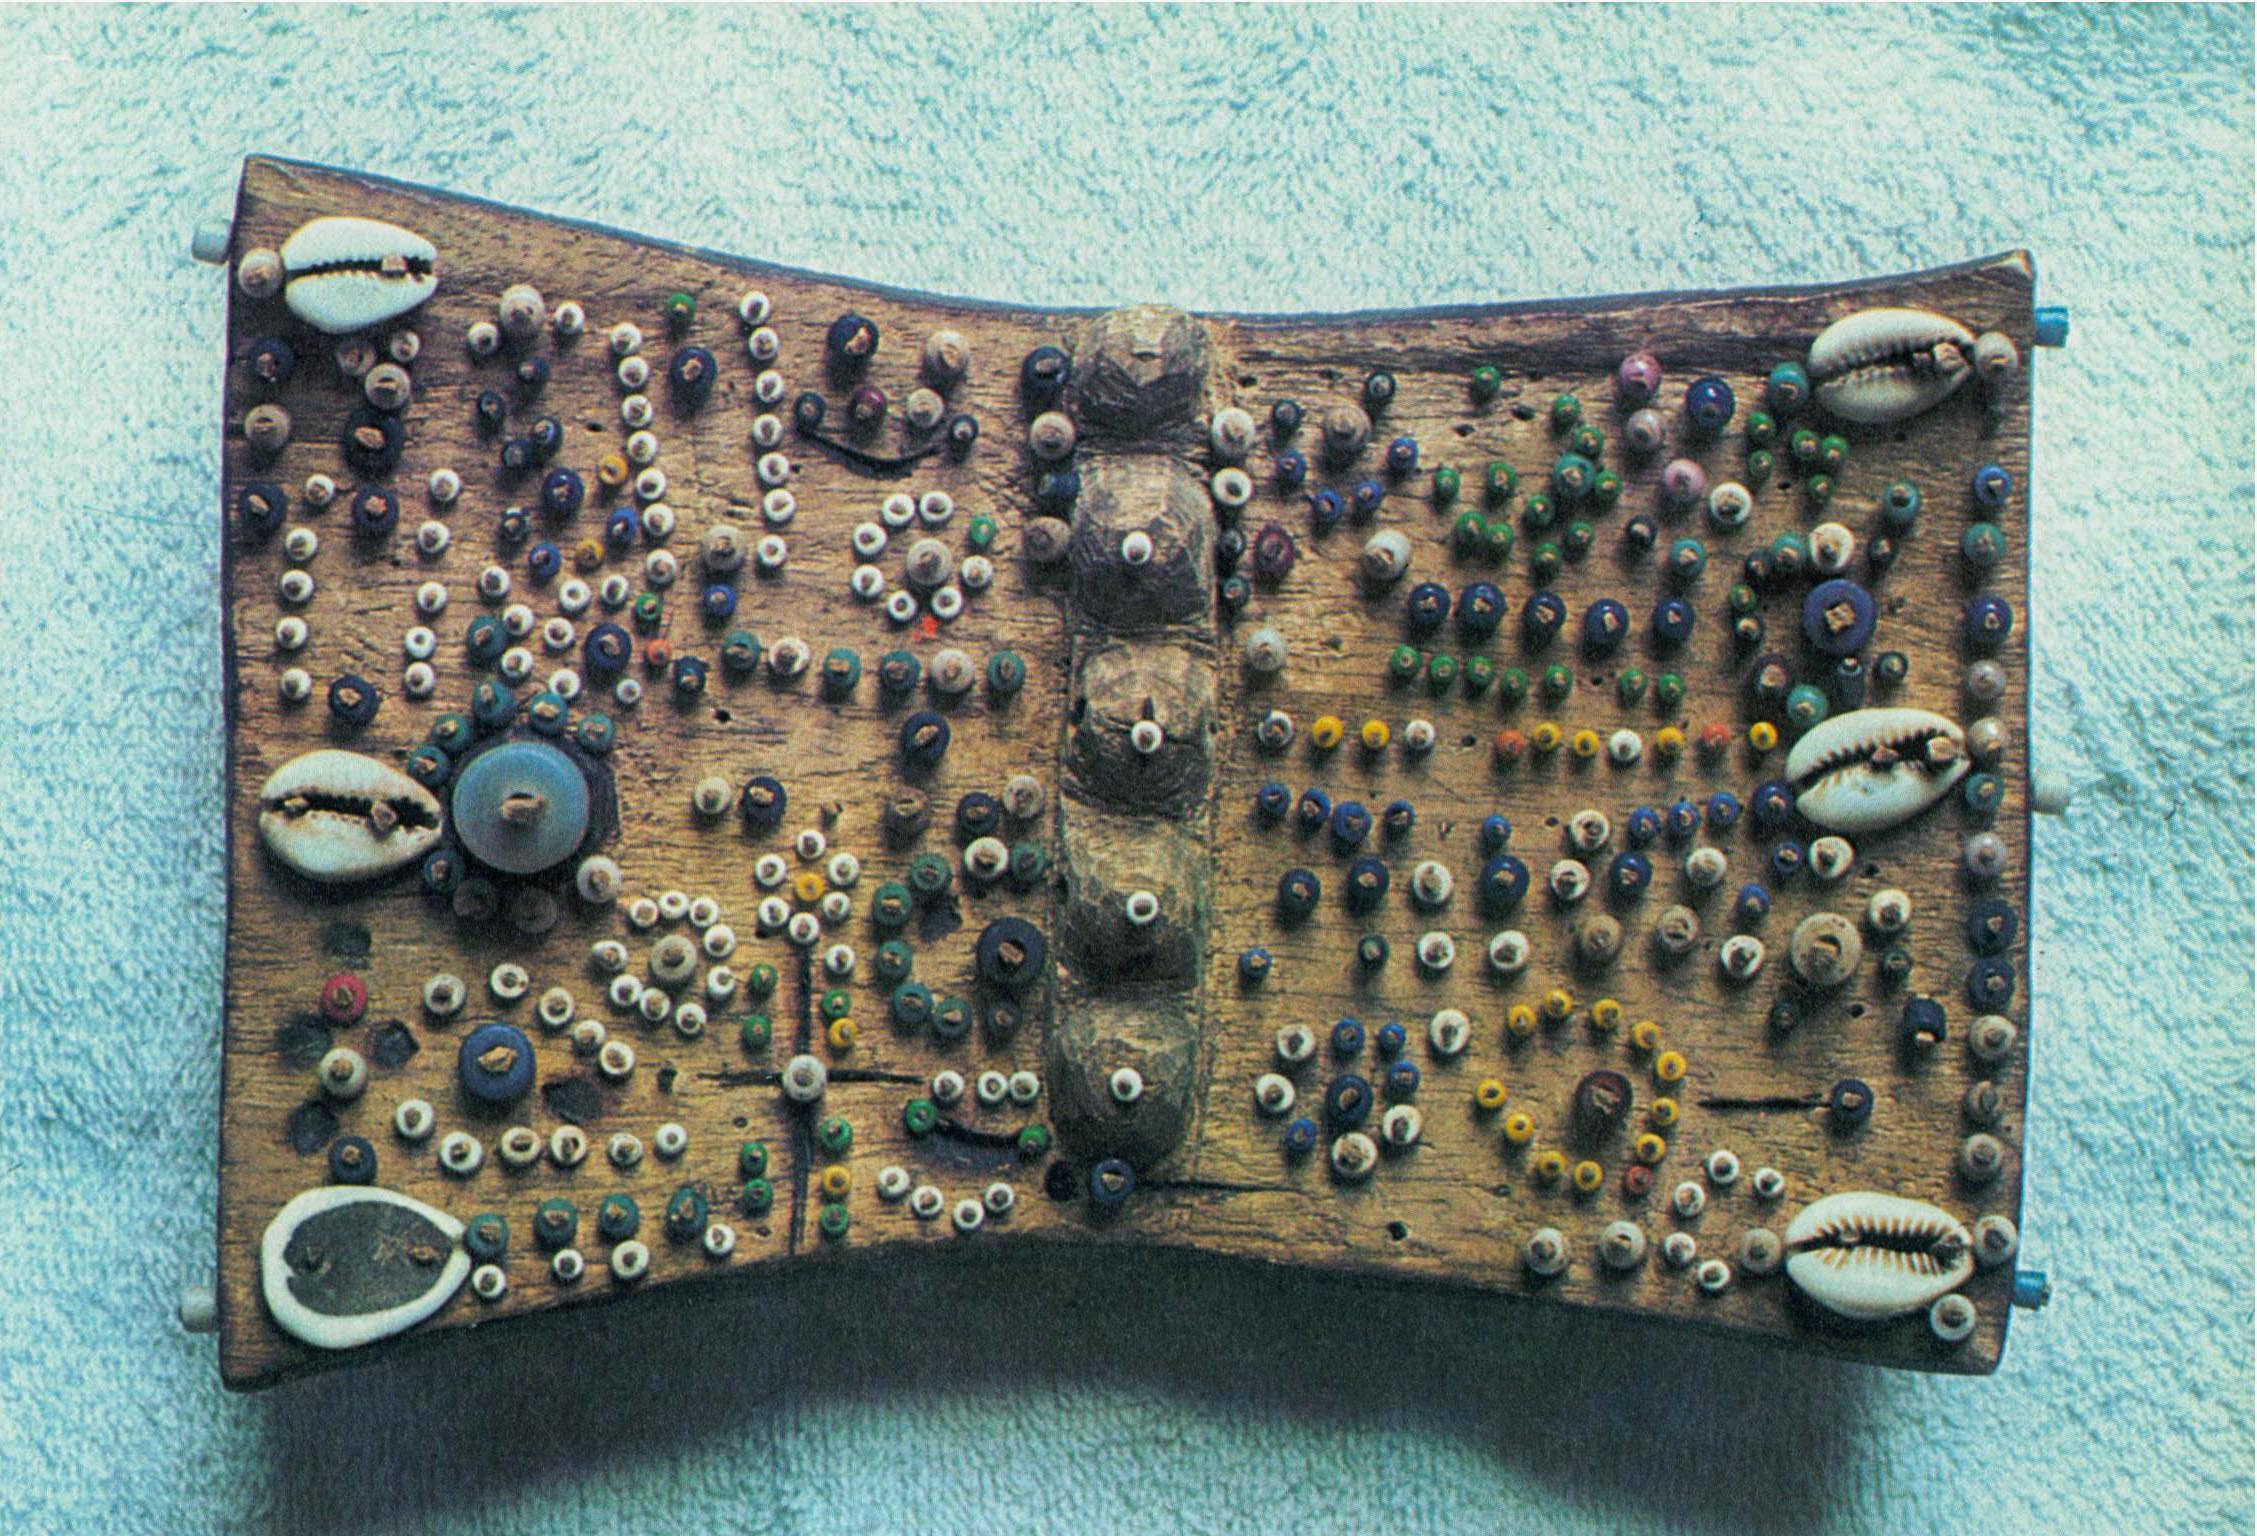
\includegraphics[width=0.6\textwidth]{img/Lukasa.jpg}
                \caption{Η συσκευή λουκάσα}
            \end{figure}
            
            Άλλοι πολιτισμοί όπως οι Ίνκα χρησιμοποιούσαν συσκευές όπως το \textit{κουίπου} \linebreak (quipu), μια κατασκευή με χορδές από βαμβάκι με κατηγοροποιημένες πληροφορίες βάσει χρώματος, διάταξης και αριθμού. Οι Ίνκα δημιουργούσαν κόμπους στις χορδές και τις χρησιμοποιούσαν για τη συλλογή και παρακολούθηση των υποχρεώσεών τους ή και για την αποθήκευση άλλων πληροφοριών όπως δεδομένα απογραφής, φορολογικών υποχρεώσεων και άλλα. \cite{Quipu}

            \begin{figure}[H] \noindent \centering
                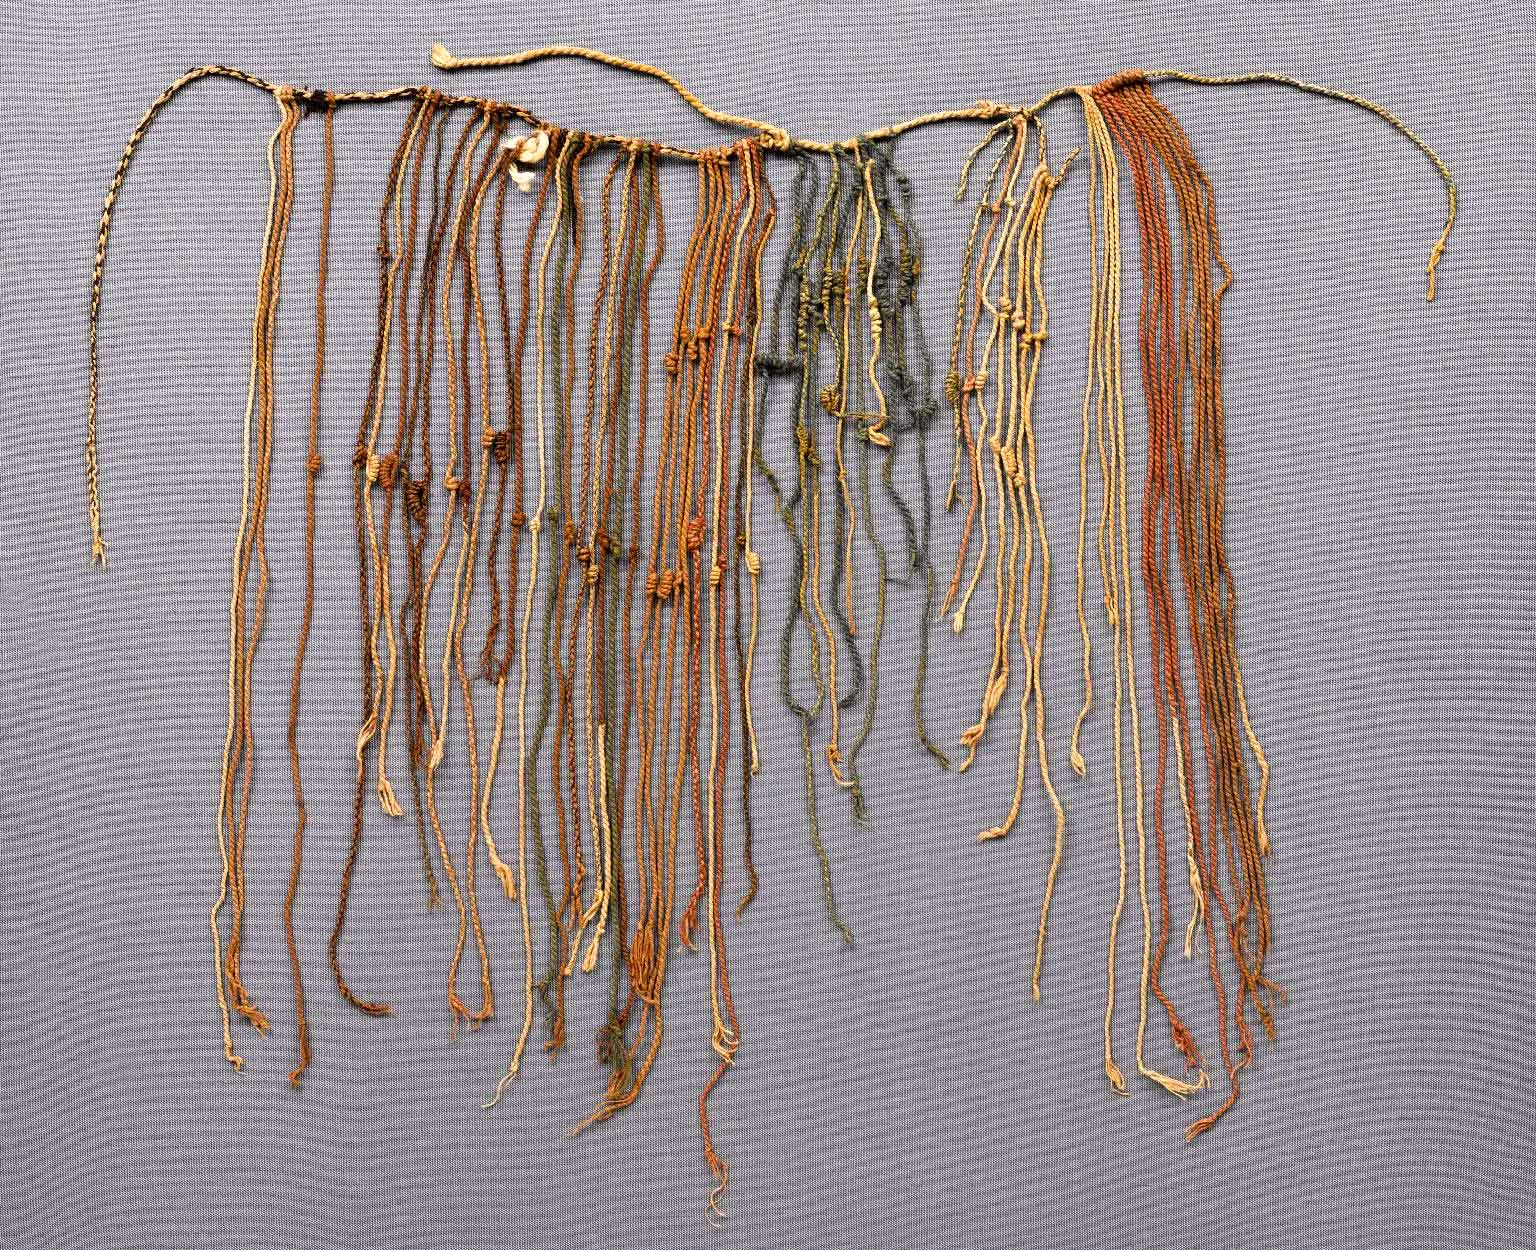
\includegraphics[width=0.5\textwidth]{img/Quipo.jpg}
                \caption{Η συσκευή κουίπου}
            \end{figure}

        \subsection{Πρώτα ημερολόγια}
            Κατασκευές όπως τα ηλιακά ρολόγια επέτρεψαν στους πληθυσμούς να διαιρέσουν την ημέρα σε τμήματα, που οδήγησε στον διαχωρισμό μεταξύ υποχρεώσεων και ελεύθερου χρόνου, ενώ με κάποιες πρώιμες προσπάθειες δημιουργίας ημερολογίων (κυρίως από Ρωμαίους, Αιγυπτίους και Μάγια) έγινε εφικτός ο διαχωρισμός του χρόνου σε διαφορετικές περιόδους για την γεωργία, τις θρησκευτικές τελετές και τις υπόλοιπες τελετουργίες, οδηγώντας έτσι σε μια μορφή διαχείρισης έργων και χρόνου. \cite{Richards_2000}

        \subsection{Σύγχρονη εποχή}
            Οι άνθρωποι διαχειρίζονται την εργασία τους εδώ και εκατοντάδες χρόνια, και μπορούμε να εντοπίσουμε τις πρώτες απόπειρες τυποποίησης αυτής της διαχείρισης από τον 18ο αιώνα. Στα τέλη του 19ου αιώνα, ανερχόμενα έργα μεγάλης κλίμακας επέφεραν την ανάγκη για μια πιο λεπτομερή διαχείριση των εργασιών, άμεση απόρροια των αυξανόμενων απαιτήσεων που θα προέκυπταν. Όμως η οργάνωση χιλιάδων εργατών και η επεξεργασία τεράστιων ποσοτήτων από πρώτες ύλες δεν θα μπορούσε να πραγματοποιηθεί επιτυχώς με τις υπάρχουσες τεχνικές.
           
            Μηχανικοί όπως ο Henry Gantt για να αντιμετωπίσουν αυτές τις ανάγκες εισήγαγαν νέες μεθόδους οργάνωσης όπως το \textbf{διάγραμμα Γκαντ}. Πρόκειται για ένα διάγραμμα αναπαράστασης όλων των επιμέρους εργασιών ενός έργου ανά το χρόνο και παρέχει μια σαφή εικόνα όλων των  διαφορετικών φάσεων, επιτρέποντας τον προσδιορισμό της κρίσιμης διαδρομής του. Επομένως είναι μια εξαιρετικά χρήσιμη μέθοδος για τον σωστό χρονοπρογραμματισμό σε τέτοια μεγέθη μεγάλης κλίμακας. Το διάγραμμα Γκαντ χρησιμοποιήθηκαν κατά κόρον σε μεγάλα έργα υποδομών όπως η Διώρυγα του Παναμά ή το φράγμα Χούβερ. \cite{strefapmiHooverGreatest}
            
            Αυτά τα νέα μεθοδολογικά εργαλεία ενέπνευσαν νέες έρευνες όπως το Πρότζεκτ Μανχάταν (Manhattan Project), τις προσπάθειες των Αμερικανών για το σχεδιασμό πυρηνικών όπλων. Για την επίτευξη αυτού του σκοπού αναπτυχτήκαν δύο νέα μοντέλα, το PERT (Program Evaluation and Review Technique) και το CPM (Critical Path Method). \cite{SaylorAcademyProjectManagement}
            
    \section{Η συνδρομή της τεχνολογίας}
        Από την δεκαετία του '60 και μετά, οι επιχειρήσεις άρχισαν να αντιλαμβάνουν τα οφέλη από τη μεθοδική οργάνωση της εργασίας. Η ψηφιακή επανάσταση που ακολούθησε δεν θα μπορούσε παρά να γιγαντώσει αυτή τη νέα πραγματικότητα.
    
        \subsection{Ψηφιακά εργαλεία}
            Με την εξέλιξη της τεχνολογίας, οι σημειώσεις και η οργάνωση μεταφέρθηκε από τις χειρόγραφες σημειώσεις, τα ημερολόγια και τα έγγραφα των γραφομηχανών σε ψηφιακά εργαλεία όπως υπολογιστικά φύλλα και προγράμματα σαν το Microsoft Project, σχεδιασμένα αποκλειστικά με σκοπό την αποτελεσματική διαχείριση έργων. 

            \subsubsection{Microsoft Project}
                \begin{figure}[H] \noindent \centering
                    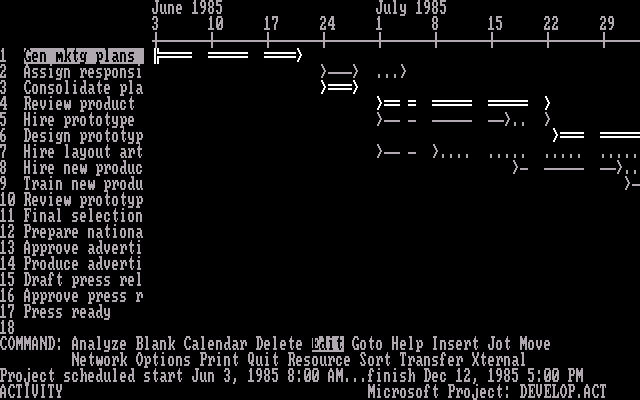
\includegraphics[width=0.7\textwidth]{img/MicrosoftProject3.png}
                    \caption{\centering Στιγμιότυπο από το Microsoft Project 3.0 (σε DOS) \cite{WinWorld}}
                \end{figure}
                
                \begin{figure}[H] \noindent \centering
                    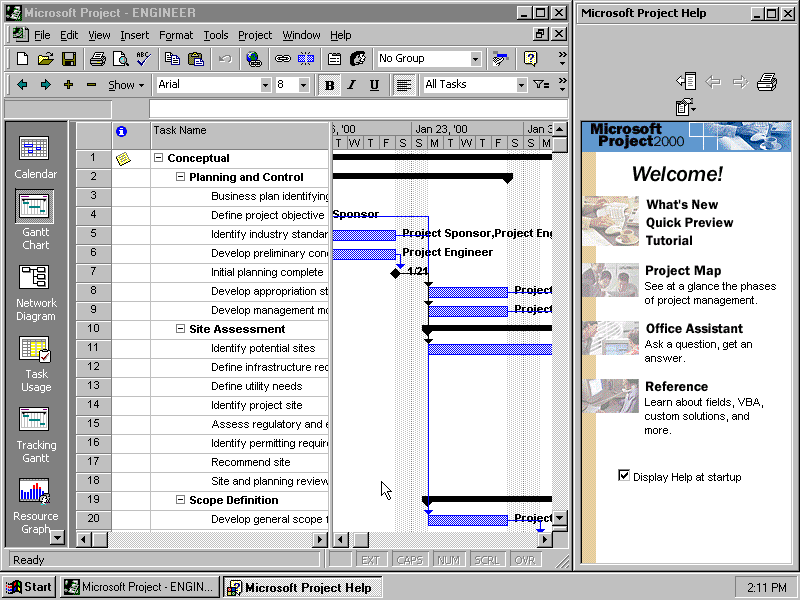
\includegraphics[width=0.7\textwidth]{img/MicrosoftProject2000.png}
                    \caption{\centering Στιγμιότυπο από το Microsoft Project 2000 \cite{WinWorld}}
                \end{figure}
                
                Πρόκειται για ένα από τα πρώτα λογισμικά διαχείρισης έργων, σχεδιασμένα για το κοινό. Η ιδέα για την δημιουργία του προήλθε από μια φάρσα του Ron Bredehoeft, ο οποίος ήθελε να εκφράσει την συνταγή για τα αυγά μπένεντικτ σε όρους διαχείρισης έργων. Παρουσιάστηκε για πρώτη φορά το 1984 ως μια DOS εφαρμογή και πλέον έχει γίνει ένα καθιερωμένο εργαλείο σε όλες τις βιομηχανίες για την οργάνωση, τον προγραμματισμό και την παρακολούθηση της προόδου των έργων.
                
                Η κεντρική οθόνη του Microsoft Project χωρίζεται σε δύο περιοχές: το διάγραμμα Γκαντ και τον πίνακα που εισάγονται οι εργασίες (input table). Υπάρχει η δυνατότητα ιεράρχησης των εργασιών με την τοποθέτηση εσοχών (indents), η δημιουργία εξαρτήσεων με το καθορισμό προκατόχων (predecessors -- μια εργασία μπορεί να ξεκινήσει να εκτελείται μόνο όταν τελειώσει ο προκάτοχός της) και η δυνατότητα αυτόματου προγραμματισμού των εργασιών, λαμβάνοντας υπόψιν τις εξαρτήσεις τους. Επιπλέον μπορούν να δημιουργηθούν αλυσιδωτές εργασίες (η μια εργασία εκτελείται μετά την άλλη), ενώ επίσης μπορούν να ανατεθούν πόροι (resources) για κάθε εργασία. Κάθε χαρακτηριστικό μπορεί να τροποποιηθεί δυναμικά, είναι εφικτή η αποτύπωση των εργασιών πέρα από το διάγραμμα Γκαντ και σε μορφή ημερολογίου, φύλλου εργασίας (task sheet) κ.α., όπως επίσης και η δημιουργία στατιστικών.

                    
    \section{Μεθοδολογίες}
       
        \subsection{Διάγραμμα Γκαντ}
            Το \textbf{διάγραμμα Γκαντ} (Gantt chart) είναι μια δισδιάστατη γραφική απεικόνιση ενός έργου, με τον οριζόντιο άξονα να αποτελεί τον χρόνο (συχνά χωρισμένο σε διαστήματα ημερών, μηνών, χρόνων) και τον κατακόρυφο άξονα να αποτελεί τις διαφορετικές εργασίες που απαρτίζουν το έργο.

            Πρόκειται για ένα πολύ σημαντικό εργαλείο καθώς δείχνει οπτικά τον χρόνο που εκτιμάται ότι θα χρειαστεί κάθε τμήμα ενός έργου, επομένως μπορεί εύκολα να χρησιμοποιηθεί για την παρακολούθηση της προόδου όλων των επιμέρους εργασιών. Έτσι, αν κάποια ξεφεύγει από το ορισμένο χρονοδιάγραμμα, μπορούν άμεσα να γίνουν οι απαραίτητες ενέργειες που χρειάζονται. \cite{Xenos}

            Για τον σχεδιασμό ενός διαγράμματος Γκαντ είναι απαραίτητος ο αρχικός διαχωρισμός των επιμέρους εργασιών, όπως επίσης και μια εκτίμηση της χρονικής διάρκειάς τους. Στην συνέχεια οι εργασίες τοποθετούνται συνήθως με σειρά ώστε αυτές που τελειώνουν νωρίτερα να βρίσκονται ψηλότερα.
            
            Γενικά είναι μια εύκολη και γρήγορη κατασκευή που απεικονίζει με σαφήνεια τη χρονική διάρκεια και την αλληλουχία των εργασιών, αλλά από την άλλη δεν μπορεί να απεικονίσει τις εξαρτήσεις μεταξύ των επιμέρους εργασιών. Έτσι δεν είναι εμφανές ποιες εργασίες πρέπει να ολοκληρωθούν πρώτα ώστε να είναι εφικτή η εκτέλεση μιας επόμενης εργασίας, και επίσης δεν αναπαρίσταται η επίδραση μιας καθυστέρησης σε κάποια φάση του έργου. Τέλος, λόγω της στατικής του δομής, δεν δύναται να αναπροσαρμοστεί σε μεταβολές στη χρονική διάρκεια εκτέλεσης κάποιας εργασίας.

        \subsection{Program evaluation and review technique (PERT)}


        \subsection{Μέθοδος κρίσιμης διαδρομής (Critical Path Method -- CPM)}


        \subsection{Agile και Kanban}


    \section{Διαχείριση έργων στο πανεπιστήμιο}
        \subsection{Προβλήματα διαχείρισης που αντιμετωπίζουν οι φοιτητές}
            % Εισαγωγική παράγραφος
            
            Σε έρευνα \cite{Fukuzawa2015} που διεξήχθη στο Πανεπιστήμιο του Τσουκούμπα της Ιαπωνίας, η οποία διερευνούσε τη διαχείριση του προγραμματισμού των εργασιών από τη πλευρά των φοιτητών, παρατηρήθηκε πως η πλειοψηφία τους αντιμετωπίζει δυσκολίες στην εκκίνηση μιας νέας εργασίας με βασικούς λόγους: α) την έλλειψη χρόνου (26,9\%), β) την αγνόησή της επειδή τη θεωρούσαν ελάσσονος σημασίας (15,7\%), γ) επειδή την ξέχασαν (12,3\%), δ) λόγω κακής συνεργασίας (11,2\%) και ε) επειδή ήταν κουραστική (8,9\%). Παρατηρούμε πως οι τρεις πρώτοι λόγοι --που καλύπτουν το μεγαλύτερο ποσοστό (54,9\%) των λόγων-- αφορούν θέματα κακής οργάνωσης από την πλευρά των φοιτητών.
           
            Σε διαφορετική έρευνα \cite{Trujillo2020}, πάλι παρουσιάζεται πως το κυριότερο πρόβλημα που αντιμετωπίζουν οι φοιτητές είναι η σωστή δόμηση του προγράμματός τους. Συνήθως ο τρόπος διαβάσματός τους καθοδηγείται από τις ίδιες τις εργασίες που έχουν να κάνουν, μιας και μόνο αυτές έχουν καταληκτικές ημερομηνίες παράδοσης, και έτσι παραμελούν τα υπόλοιπα καθήκοντα που έχουν, όπως το να παρακολουθούν τις διαλέξεις.

            Όλα αυτά μας οδηγούν στο συμπέρασμα πως είναι απαραίτητος ένας αποτελεσματικός τρόπος προγραμματισμού και διαχείρισης των εργασιών τους.

        \subsection{Χαρακτηριστικά που οι φοιτητές θα επιθυμούσαν σε μια εφαρμογή}
            Σε έρευνα \cite{Trujillo2020} που πραγματοποιήθηκε στο τμήμα Πληροφορικής του Πανεπιστημίου του Εδιμβούργου, διαπιστώθηκε πως η πλειοψηφία της ακαδημαϊκής κοινότητας επιθυμεί μια εφαρμογή διαχείρισης εργασιών να διαθέτει ημερολόγιο (θεώρησαν σημαντικό να είναι καταγραμμένες οι ημερομηνίες έναρξης/λήξης για κάθε εργασία για τη σωστή οργάνωση, όπως επίσης και χρωματική ταξινόμηση (color-coding) των εργασιών), ειδοποιήσεις / γνωστοποιήσεις για τις εργασίες και to-do λίστες (με ιεράρχιση, ομαδοποίηση και δυνατότητα εμφάνισης μπάρας προόδου). Επίσης εκφράστηκε ενδιαφέρον για τη δημιουργία ενός συστήματος ανταμοιβής, με σκοπό την ενθάρρυνση των φοιτητών να ολοκληρώνουν εργασίες.